\RequirePackage{fix-cm}
\RequirePackage{amsmath}  % for \text in math formulas: 
\RequirePackage{graphicx}

\documentclass[smallextended]{svjour3} 


\usepackage[T1]{fontenc}
%\usepackage[utf8]{inputenc}

\usepackage{csquotes}
\usepackage{hyperref} % \url
\usepackage{gensymb}  % \degree
\usepackage{multirow}
\usepackage{xr}       % cross-references to supplementary
\usepackage{float}
\usepackage{xfrac}
\usepackage[dvipsnames]{xcolor}
%\usepackage{array}
%\usepackage{hhline}
%\usepackage{makecell}

%\renewcommand\cellgape{\Gape[6pt]}
%\renewcommand\theadfont{\itshape}

% special stuff for xr package, copied from here: 
% https://www.overleaf.com/learn/how-to/Cross_referencing_with_the_xr_package_in_Overleaf
\makeatletter
\newcommand*{\addFileDependency}[1]{% argument=file name and extension
  \typeout{(#1)}
  \@addtofilelist{#1}
  \IfFileExists{#1}{}{\typeout{No file #1.}}
}
\makeatother
\newcommand*{\supplementary}[1]{%
    \externaldocument{#1}%
    \addFileDependency{#1.tex}%
    \addFileDependency{#1.aux}%
}
\newcommand*{\maintext}[1]{%
    \externaldocument{#1}%
    \addFileDependency{#1.tex}%
    \addFileDependency{#1.aux}%
}
% end of stuff for xf/supplementary

\newcommand{\SVETE}{\color{Brown}}
%\newcommand{\SVETE}{{}}

%\newcommand{\ORANGE}[1]{\colorbox{BurntOrange}{#1}}

\newcommand{\tabhline}{\noalign{\smallskip}\hline\noalign{\smallskip}}

\newcommand*{\gtwoXY}[2]{\ensuremath{\Gamma_\text{2{#2}}^\text{#1}}}
\newcommand*{\gtwoY}[1]{\ensuremath{\Gamma_\text{2{#1}}}}
\newcommand{\Hfirst}{\ensuremath{\text{H}}}
\newcommand{\Hprime}{\ensuremath{\text{H}'}}
\newcommand{\Hone}{\ensuremath{\text{H}^1}}
\newcommand{\Htwo}{\ensuremath{\text{H}^2}}
\newcommand{\gtwo}{\ensuremath{\Gamma_2}}
\newcommand{\gtwoCSA}{\ensuremath{\Gamma_2^c}}
\newcommand{\gtwoXH}{\ensuremath{\Gamma_{\text{2XH,XH}'}}}
\newcommand{\gtwoCH}{\ensuremath{\Gamma_{\text{2CH,CH}'}}}
\newcommand{\gtwoNH}{\ensuremath{\Gamma_{\text{2NH,NH}'}}}
\newcommand{\gtwoXHa}{\ensuremath{\Gamma_\text{2XH,XH}}}
\newcommand{\gtwoCHa}{\ensuremath{\Gamma_\text{2CH,CH}}}
\newcommand{\gtwoNHa}{\ensuremath{\Gamma_\text{2NH,NH}}}
\newcommand{\gtwoNNH}{\ensuremath{\Gamma_\text{2N,NH}}}
\newcommand{\gtwoCCH}{\ensuremath{\Gamma_\text{2C,CH}}}
\newcommand{\gtwoXXH}{\ensuremath{\Gamma_\text{2X,XH}}}
\newcommand{\gtwoNNHp}{\ensuremath{\Gamma_{\text{2N,NH}'}}}
\newcommand{\gtwoCCHp}{\ensuremath{\Gamma_{\text{2C,CH}'}}}
\newcommand{\gtwoXXHp}{\ensuremath{\Gamma_{\text{2X,XH}'}}}

\newcommand{\StwoCH}{\ensuremath{S^2_\text{CH}}}
\newcommand{\StwoNH}{\ensuremath{S^2_\text{NH}}}
\newcommand{\StwoXH}{\ensuremath{S^2_\text{XH}}}
\newcommand{\StwoCHp}{\ensuremath{S^2_{\text{CH,CH}'}}}
\newcommand{\StwoNHp}{\ensuremath{S^2_{\text{NH,NH}'}}}
\newcommand{\StwoXHp}{\ensuremath{S^2_{\text{XH,XH}'}}}
\newcommand{\StwoCCH}{\ensuremath{S^2_\text{C,CH}}}
\newcommand{\StwoNNH}{\ensuremath{S^2_\text{C,NH}}}
\newcommand{\StwoXXH}{\ensuremath{S^2_\text{X,XH}}}

\newcommand{\JCH}{\ensuremath{J_{\text{CH,CH}'}}}
\newcommand{\JNH}{\ensuremath{J_{\text{NH,NH}'}}}
\newcommand{\JXH}{\ensuremath{J_{\text{XH,XH}'}}}
\newcommand{\JCCH}{\ensuremath{J_{\text{C,CH}}}}
\newcommand{\JNNH}{\ensuremath{J_{\text{N,NH}}}}
\newcommand{\JXXH}{\ensuremath{J_{\text{X,XH}}}}
\newcommand{\JHH}{\ensuremath{J_\text{HH}}}
\newcommand{\Jx}{\ensuremath{J_{\text{X}}}}
\newcommand{\Jxh}{\ensuremath{J_{\text{XH}}}}

\newcommand{\nclab}{\ensuremath{{}^{13}\text{C}/{}^{15}\text{N}}}
\newcommand{\nlab}{\ensuremath{{}^{15}\text{N}}}
\newcommand{\clab}{\ensuremath{{}^{13}\text{C}}}
\newcommand{\cnolab}{\ensuremath{{}^{12}\text{C}}}
\newcommand{\hlab}{\ensuremath{{}^{1}\text{H}}}
\newcommand{\dlab}{\ensuremath{{}^{2}\text{H}}}

\newcommand{\XHtwo}{\ensuremath{\text{XH}_2}}
\newcommand{\NHtwo}{\ensuremath{\text{NH}_2}}
\newcommand{\CHtwo}{\ensuremath{\text{CH}_2}}
\newcommand{\labNHtwo}{\ensuremath{{}^{15}\text{NH}_2}}
\newcommand{\labCHtwo}{\ensuremath{{}^{13}\text{CH}_2}}
\newcommand{\CHthree}{\ensuremath{\text{CH}_3}}

\newcommand{\sigmaIS}{\ensuremath{\sigma_{\text{IS}}}}
\newcommand{\qinner}{\enquote{inner}}
\newcommand{\qouter}{\enquote{outer}}

\newcommand{\oneJch}{\ensuremath{^1\!J_\text{CH}}}
\newcommand{\oneJnh}{\ensuremath{^1\!J_\text{NH}}}
\newcommand{\oneJxh}{\ensuremath{^1\!J_\text{XH}}}
\newcommand{\oneJcc}{\ensuremath{^1\!J_{\text{CC}}}}

\newcommand{\M}{\ensuremath{\hphantom{-}}}

\newcommand{\Iinn}{\ensuremath{I_\textrm{inn}}}
\newcommand{\Iout}{\ensuremath{I_\textrm{out}}}
\newcommand{\Ioutone}{\ensuremath{I_\textrm{out1}}}
\newcommand{\Iouttwo}{\ensuremath{I_\textrm{out2}}}

\newcommand*{\Xaa}[1]{\ensuremath{\textrm{\ensuremath{#1}}^{\alpha\alpha}}}
\newcommand*{\Xab}[1]{\ensuremath{\textrm{\ensuremath{#1}}^{\alpha\beta}}}
\newcommand*{\Xba}[1]{\ensuremath{\textrm{\ensuremath{#1}}^{\beta\alpha}}}
\newcommand*{\Xabba}[1]{\ensuremath{\textrm{\ensuremath{#1}}^{\alpha\beta + \beta\alpha}}}
\newcommand*{\Xabbam}[1]{\ensuremath{\textrm{\ensuremath{#1}}^{\alpha\beta - \beta\alpha}}}
\newcommand*{\Xbb}[1]{\ensuremath{\textrm{\ensuremath{#1}}^{\beta\beta}}}

% C±(HαHβ + HβHα) 
\newcommand{\TermInner}{\ensuremath{ 
  C_\pm (
     H_\alpha H'_\beta + 
     H_\beta H'_\alpha ) }}
% C±HαHα 
\newcommand{\TermOuterA}{\ensuremath{
  C_\pm H_\alpha H'_\alpha
}}
% C±HβHβ
\newcommand{\TermOuterB}{\ensuremath{
  C_\pm H_\beta H'_\beta
}}
%C±(HαHα + C±HβHβ) 
\newcommand{\TermOuter}{\ensuremath{ 
  C_\pm (
     H_\alpha H'_\alpha + 
     H_\beta H'_\beta ) }}
  



\makeatletter
\renewcommand{\theequation}{S\arabic{equation}}
\renewcommand{\thefigure}{S\arabic{figure}}
\renewcommand{\thetable}{S\arabic{table}}
%\renewcommand{\bibnumfmt}[1]{[S#1]}
%\renewcommand{\citenumfont}[1]{S#1}
\makeatother

\maintext{G2_Method}

\journalname{Journal of Biomolecular NMR}
%

\begin{document}

\title{
  Accurate measurement of dipole\slash dipole transverse 
  cross-correlated relaxation \gtwo{} in methylenes and primary 
  amines of uniformly \nclab-labeled proteins
}

\subtitle{{SUPPLEMENTARY~INFORMATION}}
\titlerunning{SUPPLEMENTARY: Accurate measurement of \gtwo}      

\author{Dmitry M. Lesovoy 
        \thanks{corresponding author, e-mail:  lesovoydm@gmail.com} \and
        Maxim A. Dubinnyi      \and 
        Svetlana B. Nolde      \and 
        Eduard V. Bocharov  
          \thanks{corresponding author, e-mail:  bon@nmr.ru}\and 
        Alexander S. Arseniev
}

\institute{
  Dmitry M. Lesovoy    \and 
  Maxim A. Dubinnyi    \and 
  Svetlana B. Nolde    \and 
  Eduard V. Bocharov   \and 
  Alexander S. Arseniev
  \at
  Shemyakin{-}Ovchinnikov Institute of Bioorganic Chemistry, 
  Russian Academy of Sciences RAS,  Str. Miklukho{‐}Maklaya 
  16/10, Moscow, 117997, Russian Federation \\
\and
  Maxim A. Dubinnyi    \and 
  Eduard V. Bocharov   \and 
  Alexander S. Arseniev \at
  Moscow Institute of Physics and Technology (State University), 
  Institutsky per., 9, Dolgoprudny, 141700, Russian Federation  
}

\date{Received: date / Accepted: date}

\maketitle

\newpage
The \oneJch-modulated approach illustrated by Fig. \ref{fig:scheme3} 
      can be similarly applied to modify the {CC(CO)NH} {TOCSY} based 
      scheme, which has been used earlier as a \oneJch-resolved approach
      \cite{zheng_measurement_2004}. Fig. S1 illustrates a modification of
      this pulse sequence affecting only the period preceding \clab{} 
      {FLOPSY}:
\begin{figure}
    \centering
    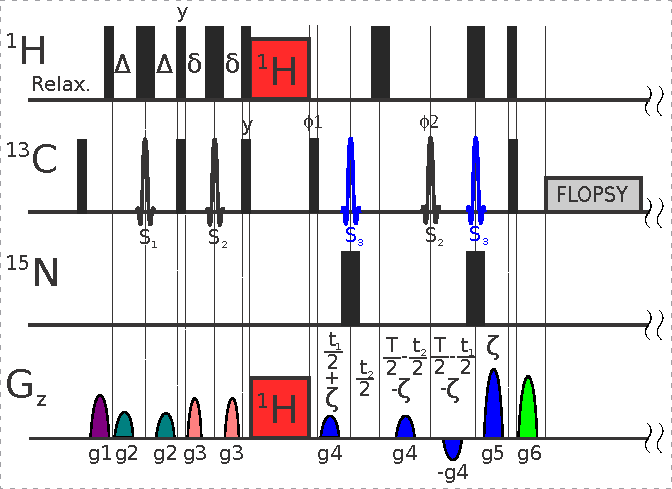
\includegraphics{FigS1}
    \caption{
       The modification of the 3D \oneJch-resolved pulse sequence (Zheng and Yang 2004) into \oneJch-modulated approach. All the adjustments take place only before \clab{}-FLOPSY of the CC(CO)NH TOCSY scheme. Narrow and thick bars represent 90\degree{} and 180\degree{} pulses. Constant-time \clab{} States-TPPI sampling is implemented with the aid of $t_1$ delay and $\varphi_1$; INEPT delays are $\Delta = 2\delta = 1/(4\oneJch)$; transverse relaxation delay $T$ is 28.6 ms; two 3D experiments are carried out with $t_2$ delays (used for \oneJch evolution) 0 and $\delta$; $\zeta = 1.2$ ms delay appears only for g5. The red box represents the same block as in Fig. 1. S1 is a 500 $\mu s$ long \clab{} inversion adiabatic Chirp pulse. S2 is a 220 $\mu s$ long 180\degree{} Q3 pulse (the offset at 36 ppm). S3 is a 265 $\mu s$ long inversion IBurp1 pulse (the offset at 145 ppm). Gradient pulses with squared sine shape and 1 ms length except for g3 (0.6 ms) are used. The g1-g5 gradient strengths are as follows: 27\%, 37\%, 47\%, 25\%, 75\%, 57\% whereas 100\% corresponds to 53.5 G/cm. The default phase is $x$ and the phase cycle is:
       $\varphi_1 = x, -x$;
       $\varphi_2 = 2(x), 2(-x)$;
       $\varphi_\text{REC} = 2(x, -x)$.
    }
    \label{fig:scheme4}
\end{figure}
In this case, both the \qouter{} and the \qinner{} 
      components of \clab{} triplet are transferred for detection. 
      Data processing was performed as described in Scheme
      \ref{subseq:scheme3}. Notably, equalizing the intensities of the 
      \qouter{} and \qinner{} components prior to {FLOPSY} (as in the work 
      of Zheng and Yang \cite{zheng_measurement_2004}) makes a reference
      experiment unnecessary if $A = 0$ is assumed, although doing 
      experiments at more than one value of $T$ would improve the accuracy 
      of data approximation and the obtained values of \gtwoCH.

\begin{figure}
    \centering
    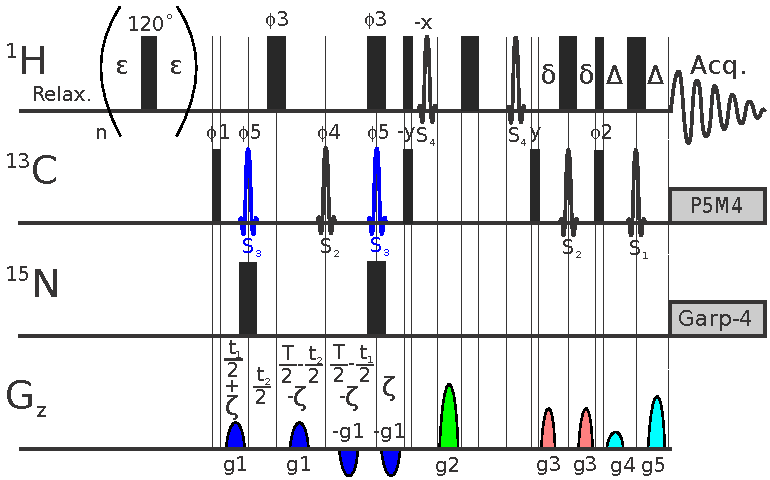
\includegraphics{FigS2}
    \caption{
        The simplification of the \oneJch-modulated Scheme \ref{subseq:scheme3} with \hlab--\clab \{NOE\} enhancement of $C_z$ magnetization. Narrow and thick bars represent 90\degree{} and 180\degree{} pulses. Constant-time \clab{} Echo-Antiecho sampling is implemented with the aid of $t_1$ delay and g1; INEPT delays are $\Delta = 2\delta = 1/(4 \oneJch)$; transverse relaxation delay $T = N*28.6$ ms; $t_2$ delay is used for \oneJch{} evolution; $\zeta = 1.2$ ms delay appears only for g1; $\epsilon = 2.5$ ms. \nlab- and \clab-decoupling are applied during acquisition. 
        S1 is a $500 \mu s$ long \clab{} inversion adiabatic Chirp pulse. 
        S2 is a $220 \mu s$ long 180\degree{} Q3 pulse (the offset at 36 ppm). S3 is a $265 \mu s$ long inversion IBurp1 pulse (the offset at 145 ppm).
        S4 is a 90\degree{} sinc-shaped water-selective \hlab{} flip-back pulse with a duration of 3 ms.
        Gradient pulses with squared sine shape and 1 ms length except for g3 (0.6 ms) are used. The g1-g5 gradient strengths are as follows: 40\%, 57\%, 47\%, 10\%, 50.2\% whereas 100\% corresponds to 53.5 G/cm.
        The default phase is $x$ and the phase cycle is: 
        $\varphi_1 = y, -y$; 
        $\varphi_2 = 2(x), 2(-x)$; 
        $\varphi_3 = 4(x), 4(-x)$; 
        $\varphi_4 = 8(x), 8(-x)$; 
        $\varphi_5 = 16(x), 16(-x)$; 
        $\varphi_\text{REC} = 8(x, -x, -x, x)$. 
        For each successive $t_1$ value, $\varphi_1$ and the phase of the receiver are incremented by 180\degree. 
    }
    \label{fig:scheme5}
\end{figure}
ggg

\begin{table*} % two column table (star *)
\caption{
Comparison of the results obtained with the aid of Schemes 1-3. 
A reference set of 20 methylene groups characterized by a good 
signal to noise ratio and the absence of signal overlap is used. 
$\Delta$ denotes corresponding errors. The table includes various 
types of methylene groups spaced differently from the backbone. 
Displayed \gtwoCH{} cover the entire typical range of values. 
The comprehensive data set of methylene groups of {NTII} has been 
deposited to the BMRB as entry 19704. \gtwoNH{} values for all nine 
\NHtwo{} groups in {NTII} are available only for Scheme 3
}

\begin{tabular}{|rl|ll|ll|ll|ll|}
\hline\noalign{\smallskip}
  \multicolumn{2}{|c|}{group} & 
  \multicolumn{2}{c|}{Scheme 1} &
  \multicolumn{2}{c|}{Scheme 2} & 
  \multicolumn{4}{c|}{Scheme 3} \\
\hline\noalign{\smallskip}
  & &
   \gtwo & $\Delta\gtwo$ &
   \gtwo & $\Delta\gtwo$ &
   \gtwo & $\Delta\gtwo$ &
   $S_2$ & $\Delta S_2$ \\

\noalign{\smallskip}\hline\noalign{\smallskip}
19G & CA  & $-5$   & 1 & $-5.4$  & 0.8 & $-5.5$  & 0.3  & $-0.20$  & 0.01 \\
41G & CA  & $-6.5$ & 1 & $-6.8$  & 0.7 & $-6.6$  & 0.3  & $-0.24$  & 0.01 \\
11P & CB  & $-4$   & 1 & $-4.3$  & 0.7 & $-4.1$  & 0.3  & $-0.15$  & 0.01 \\
12P & CG  & $+5$   & 1 & $+4.9$  & 0.5 & $+4.6$  & 0.3  & $+0.17$  & 0.01 \\
43P & CG  & $-1$   & 1 & $-1.0$  & 0.6 & $-1.1$  & 0.3  & $-0.04$  & 0.01 \\
43P & CD  & $-5.5$ & 1 & $-5.7$  & 0.7 & $-6.2$  & 0.3  & $-0.23$  & 0.01 \\
23C & CB  & $-7$   & 1 & $-6.8$  & 0.7 & $-7.4$  & 0.3  & $-0.27$  & 0.01 \\
54C & CB  & $-6.5$ & 2 & $-7.6$  & 0.6 & $-7.7$  & 0.3  & $-0.28$  & 0.01 \\
 4H & CB  & $-12$  & 2 & $-10.1$ & 0.9 & $-10.4$  & 0.6  & $-0.38$  & 0.02 \\
27W & CB  & $-10$  & 2 & $-9.7$  & 0.9 & $-10.3$  & 0.4  & $-0.38$  & 0.01 \\
35I & CG1 & $-0.5$ & 1 & $-0.7$  & 0.6 & $-0.9$  & 0.3  & $-0.03$  & 0.01 \\
51L & CB  & $-5$   & 1 & $-5.1$  & 0.6 & $-5.3$  & 0.4  & $-0.20$  & 0.01 \\
29S & CB  & $-1$   & 1 & $-0.7$  & 0.8 & $-1.3$  & 0.4  & $-0.05$  & 0.01 \\
15K & CB  & $+1$   & 1 & $-0.2$  & 0.8 & $+0.3$  & 0.3  & $+0.01$  & 0.01 \\
15K & CE  & $+1$   & 1 & $+1.2$  & 0.3 & $+0.6$  & 0.7  & $+0.02$  & 0.02 \\
26K & CE  & $+2$   & 1 & $+2.3$  & 0.3 & $+1.7$  & 0.4  & $+0.06$  & 0.01 \\
55R & CG  & $-1$   & 1 & $-0.2$  & 0.5 & $-0.9$  & 0.3  & $-0.03$  & 0.01 \\
10Q & CG  & \M$0$   & 1 & \M$0.0$  & 0.7 & $-0.2$  & 0.4  & $-0.01$  & 0.01 \\
 2E & CG  & \M$0$  & 1 & $-0.4$  & 0.5 & $-0.4$  & 0.3  & $-0.02$  & 0.01 \\
22N & CB  & $-5$   & 1 & $-5.1$  & 0.6 & $-4.9$  & 0.3  & $-0.18$  & 0.01 \\
 5N & ND2 & ---    &---&---      & --- & $-0.1$  & 0.1 & $-0.01$  & 0.02 \\
 6Q & NE2 & ---    &---&---      & --- & $-0.4$  & 0.1 & $-0.06$  & 0.02 \\
 7Q & NE2 & ---    &---&---      & --- & $-0.5$  & 0.1 & $-0.07$  & 0.01 \\
10Q & NE2 & ---    &---&---      & --- & $-0.2$  & 0.1 & $-0.03$  & 0.01 \\
22N & ND2 & ---    &---&---      & --- & $-0.7$  & 0.2 & $-0.09$  & 0.03 \\
50N & ND2 & ---    &---&---      & --- & $-0.6$  & 0.1 & $-0.08$  & 0.01 \\
52N & ND2 & ---    &---&---      & --- & $-0.6$  & 0.1 & $-0.08$  & 0.01 \\
60N & ND2 & ---    &---&---      & --- & $-1.4$  & 0.3 & $-0.19$  & 0.05 \\
61N & ND2 & ---    &---&---      & --- & $-0.9$  & 0.1 & $-0.11$  & 0.02 \\
\noalign{\smallskip}\hline
\end{tabular}
\label{tab:gtwo} 
\end{table*}

\begin{table}[]
    \caption{
       Statistics of the occurrence of methylene groups in 20 proteinogenic 
       amino acid residues and a fraction of the {NTII} methylenes with 
       successfully measured \gtwo{}. The complete set of \gtwo{} values is 
       available in the {BMRB} (data set 19704). 
    }
    \centering
    \begin{tabular}{ccccc}
      \hline\noalign{\smallskip}
      Amino acid & Methylenes & Count in NTII & 
           Methylenes in NTII & Measured \gtwoCH \\
      \tabhline
      Ala   & 0  & 0  & 0  & 0  \\
      Arg   & 3  & 4  & 12 & 12 \\
      Asn   & 1  & 6  & 6  & 6  \\
      Asp   & 1  & 2  & 2  & 2  \\
      Cys   & 1  & 8  & 8  & 8  \\
      Gln   & 2  & 3  & 6  & 6  \\
      Glu   & 2  & 3  & 6  & 6  \\
      Gly   & 1  & 5  & 5  & 5  \\
      His   & 1  & 2  & 2  & 2  \\
      Ile   & 1  & 2  & 2  & 2  \\
      Leu   & 1  & 2  & 2  & 2  \\
      Lys   & 4  & 5  & 20 & 19 \\
      Met   & 2  & 0  & 0  & 0  \\
      Phe   & 1  & 0  & 0  & 0  \\
      Pro   & 3  & 4  & 12 & 12 \\
      Ser   & 1  & 4  & 4  & 4  \\
      Thr   & 0  & 6  & 0  & 0  \\
      Trp   & 1  & 2  & 2  & 2  \\
      Tyr   & 1  & 1  & 1  & 1  \\
      Val   & 0  & 2  & 0  & 0  \\
    \tabhline
      TOTAL & 27 & 61 & 90 & 89 \\
    \noalign{\smallskip}\hline
    \end{tabular}
    \label{tab:gtwostats}
\end{table}

\begin{table}[]
    \caption{
      The values of \oneJch{} coupling constants for 26 types of
      methylene groups (out of 27, except for Phe residue)
      averaged over all methylene groups of the same type in {NTII} and \cite{lesovoy_nmr_2017}.
    }
    \centering
    \begin{tabular}{ccc}
      \hline\noalign{\smallskip}
        Residue & Atom & \oneJch{} \\
      \tabhline
        \multirow{3}{*}{Arg} 
            & CB  & $ 130.1 \pm 0.8 $ \\
            & CG  & $ 128.0 \pm 1.1 $ \\
            & CD  & $ 139.9 \pm 0.6 $ \\
      \tabhline
        Asn & CB  & $ 131.5 \pm 1.0 $\\
      \tabhline
        Asp & CB  & $ 129.2 \pm 0.9 $ \\
      \tabhline
        Cys & CB  & $ 143.5 \pm 2.6 $ \\
      \tabhline
        \multirow{2}{*}{Gln}  
            & CB  & $ 131.9 \pm 0.3 $ \\
            & CG  & $ 129.1 \pm 1.1 $ \\
      \tabhline
        \multirow{2}{*}{Glu}
            & CB  & $ 130.2 \pm 0.5 $ \\
            & CG  & $ 126.7 \pm 0.5 $ \\
      \tabhline
        Gly & CA  & $ 142.0 \pm 0.8 $ \\
      \tabhline
        His & CB  & $ 133.3 \pm 0.9 $ \\
      \tabhline
        Ile & CG1 & $ 126.3 \pm 0.3 $ \\
      \tabhline
        Leu & CB  & $ 129.3 \pm 0.8 $ \\
      \tabhline
        \multirow{4}{*}{Lys}
            & CB  & $ 129.7 \pm 0.6 $ \\
            & CG  & $ 126.8 \pm 0.5 $ \\
            & CD  & $ 128.0 \pm 0.3 $ \\
            & CE  & $ 143.1 \pm 0.5 $ \\
      \tabhline
        \multirow{2}{*}{Met}
            & CB  & $ 130.8 \pm 0.5 $ \\
            & CG  & $ 138.7 \pm 0.5 $ \\
      \tabhline
        \multirow{3}{*}{Pro}
            & CB  & $ 134.9 \pm 0.4 $ \\
            & CG  & $ 133.9 \pm 0.4 $ \\
            & CD  & $ 144.1 \pm 0.6 $ \\
      \tabhline
        Ser & CB  & $ 147.0 \pm 0.9 $ \\
      \tabhline
        Trp & CB  & $ 130.3 \pm 0.4 $ \\
      \tabhline
        Tyr & CB  & $ 133.4 \pm 0.3 $ \\
      \noalign{\smallskip}\hline
    \end{tabular}
    \label{tab:oneJch}
\end{table}

\bibliographystyle{spphys}       % APS-like style for physics
\bibliography{G2_Method}   % name your BibTeX data base

\end{document}
